% ═══════════════════════════════════════════════════════════════════════════════
% ZOMBI2 — Non-independence of gene families: from phylogenetic profiles to Potts models
% ═══════════════════════════════════════════════════════════════════════════════
\documentclass[11pt, oneside]{article}
\usepackage[T1]{fontenc}
\usepackage[margin=1in]{geometry}
\usepackage{amsmath, amssymb, amsthm}
\usepackage{booktabs}
\usepackage{xcolor}
\usepackage{tikz}
\usetikzlibrary{shapes, arrows.meta, positioning, calc}
\usepackage{hyperref}
\usepackage{enumitem}
\usepackage{tcolorbox}
\tcbuselibrary{breakable, skins}
\usepackage{fancyhdr}

\definecolor{mainblue}{RGB}{41, 54, 122}
\definecolor{maingreen}{RGB}{98, 175, 74}
\definecolor{mainred}{RGB}{183, 53, 45}
\definecolor{boxbg}{RGB}{245, 247, 252}
\definecolor{boxframe}{RGB}{41, 54, 122}
\definecolor{faqcyan}{RGB}{0, 160, 190}

\newtcolorbox{conceptbox}[1][]{colback=boxbg, colframe=boxframe, fonttitle=\bfseries,
  title=#1, breakable, sharp corners=south, boxrule=0.8pt, left=6pt, right=6pt, top=4pt, bottom=4pt,
  before upper={\parindent=0pt}}
\newtcolorbox{intuitionbox}[1][]{colback=maingreen!5, colframe=maingreen!60!black, fonttitle=\bfseries,
  title=#1, breakable, sharp corners=south, boxrule=0.8pt, left=6pt, right=6pt, top=4pt, bottom=4pt,
  before upper={\parindent=0pt}}
\newtcolorbox{warningbox}[1][]{colback=mainred!5, colframe=mainred!60!black, fonttitle=\bfseries,
  title=#1, breakable, sharp corners=south, boxrule=0.8pt, left=6pt, right=6pt, top=4pt, bottom=4pt,
  before upper={\parindent=0pt}}
\newtcolorbox{faqbox}[1][]{colback=faqcyan!5, colframe=faqcyan!60!black, fonttitle=\bfseries,
  title=#1, breakable, sharp corners=south, boxrule=0.8pt, left=6pt, right=6pt, top=4pt, bottom=4pt,
  before upper={\parindent=0pt}}

\newcommand{\sig}{\boldsymbol{\sigma}}
\newcommand{\present}{\textbf{1}}
\newcommand{\absent}{\textbf{0}}

\pagestyle{fancy}
\fancyhf{}
\fancyhead[L]{\small\textcolor{mainblue}{ZOMBI2 --- Non-independence of gene families}}
\fancyhead[R]{\small\textcolor{mainblue}{for A. Davín}}
\fancyfoot[C]{\thepage}
\renewcommand{\headrulewidth}{0.4pt}

\title{\vspace{-1.4cm}
  {\Large \textcolor{mainblue}{\textsc{Non-independence of gene families}}}\\[0.3em]
  {\large From phylogenetic profiles to Potts models --- and how to simulate them in ZOMBI2}\\[0.4em]
  {\normalsize A chalk-talk for the ZOMBI2 project}}
\author{}
\date{\today}

\begin{document}
\maketitle
\thispagestyle{fancy}
\vspace{-0.8cm}

\begin{abstract}\noindent
Gene families do not evolve independently: those that work together --- in the same pathway
or complex --- tend to be present or absent \emph{together} across genomes. This document
explains (1) the empirical result and its exploitation for function prediction (Pellegrini
1999; Croce 2019; Fukunaga \& Iwasaki 2022, the papers Gergely suggested); (2) the physics
those methods borrow --- the Ising and Potts models --- with intuition first and math second;
and (3) three concrete ways to \emph{generate} this non-independence in ZOMBI2, mapped onto
the rate-model seam we already have, plus a clean validation test. The goal is a shared
picture precise enough to argue about design choices.
\end{abstract}

% ═══════════════════════════════════════════════════════════════════════════════
\section{Why this matters, and a running example}
% ═══════════════════════════════════════════════════════════════════════════════

A \emph{phylogenetic profile} of a gene family is the binary string of its
presence/absence across a set of genomes. Line up many families as rows and many species as
columns and you get a presence/absence matrix. The central empirical fact: \emph{rows that
look alike tend to be functionally related}. Our current ZOMBI2 already emits exactly this
matrix (\texttt{Profiles.tsv}) --- but it emits it from \emph{independent} per-family
birth--death processes, so its rows are only correlated through the shared species tree, never
through function. Making that correlation real is the scientific heart of ZOMBI2.

\begin{intuitionbox}[The commuting analogy]
Two colleagues who are always in the office on the same days are probably on the same team.
You don't need to know what they do --- their \emph{attendance pattern} betrays the coupling.
Phylogenetic profiling is this idea for genes: a gene's ``attendance record'' across genomes,
compared to every other gene's, reveals who works with whom. The subtlety (Part~3 below) is
telling a real team apart from two people who merely happen to live in the same city.
\end{intuitionbox}

\begin{conceptbox}[Toy example we will reuse]
Four gene families across six species. Families $A$ and $B$ are in one pathway (they
co-occur); $C$ is unrelated; $D$ is a ``hub'' present almost everywhere.
\begin{center}\small
\begin{tabular}{lcccccc}
\toprule
family & $s_1$ & $s_2$ & $s_3$ & $s_4$ & $s_5$ & $s_6$ \\
\midrule
$A$ & 1 & 1 & 1 & 1 & 0 & 0 \\
$B$ & 1 & 1 & 1 & 1 & 0 & 0 \\
$C$ & 1 & 0 & 1 & 0 & 1 & 0 \\
$D$ & 1 & 1 & 1 & 1 & 1 & 0 \\
\bottomrule
\end{tabular}
\end{center}
$A$ and $B$ have \emph{identical} profiles $\Rightarrow$ strong coupling. $C$'s profile looks
random relative to $A$ $\Rightarrow$ no coupling. $D$ is almost always present, so it carries
little information on its own.
\end{conceptbox}

% ═══════════════════════════════════════════════════════════════════════════════
\section{What the three papers found}
% ═══════════════════════════════════════════════════════════════════════════════

\textbf{Pellegrini et al.\ (1999), PNAS --- the original idea.} They built binary profiles for
every protein across the (then $\sim$16) fully sequenced genomes and grouped proteins by
profile similarity (Hamming distance). Proteins with similar profiles were disproportionately
in the same pathway or complex (ribosome, flagellum, biosynthesis routes). The logic is
selective: if a pathway is useless to a lineage, \emph{all} its members tend to be lost
together; if it is essential, all are retained. In our toy data, $A$ and $B$ would be grouped;
$C$ would not.

\textbf{Croce et al.\ (2019), PLoS Comput.\ Biol.\ --- direct couplings, and two scales.}
Simple profile similarity has a well-known flaw (Part~3): if $A$--$B$ and $B$--$D$ both
co-occur, then $A$--$D$ will look correlated even if they never interact. Croce et al.\ apply
\emph{Direct Coupling Analysis} (DCA), which fits a global Potts model to the whole matrix and
reports \emph{direct} couplings $J_{ij}$ with the indirect ones subtracted out
(``\emph{PhyDCA}''). Their second idea is \emph{multi-scale}: a genome-level phyletic coupling
between two protein domains, \emph{plus} a residue-level coevolution signal (classic DCA on a
multiple-sequence alignment) between the same two domains, is much stronger evidence of a real
physical interaction than either scale alone.

\textbf{Fukunaga \& Iwasaki (2022), Bioinformatics --- inverse Potts beats correlation.} They
show, on function-prediction benchmarks, that the inverse-Potts (DCA) couplings predict
functional links substantially better than pairwise correlation or mutual information ---
precisely because they remove indirect (transitive) associations. They also tackle the
\emph{phylogenetic} confounder by working with reconstructed gain/loss events on tree branches
rather than raw presence/absence, which de-weights correlations that are just shared ancestry.

\begin{faqbox}[Quick questions]
\textbf{Q: Isn't this just clustering rows?} For Pellegrini, essentially yes. The 2019/2022
advances are (i) replacing ``rows look alike'' with a \emph{generative} model that separates
direct from indirect coupling, and (ii) correcting for the tree.\\[2pt]
\textbf{Q: Why do we (ZOMBI2) care what the inference methods do?} Because they define our
\emph{target}. If we can inject a coupling and have their method recover it, our simulator
produces data with the right statistical structure --- which is exactly what these fields lack
for benchmarking.
\end{faqbox}

% ═══════════════════════════════════════════════════════════════════════════════
\section{The physics: Ising, then Potts}
% ═══════════════════════════════════════════════════════════════════════════════

\textbf{Ising (two states).} Imagine each gene family $i$ is a switch $\sigma_i\in\{0,1\}$
(absent/present) in one genome. Attach to each switch a \emph{field} $h_i$ (its intrinsic
tendency to be on) and to each pair a \emph{coupling} $J_{ij}$ (how much they like to agree).
Define an \emph{energy}
\[
E(\sig) \;=\; -\sum_i h_i\,\sigma_i \;-\; \sum_{i<j} J_{ij}\,\sigma_i\sigma_j ,
\qquad
P(\sig) \;=\; \frac{1}{Z}\,e^{-E(\sig)} \;=\; \frac{1}{Z}\,
\exp\!\Big(\textstyle\sum_i h_i\sigma_i + \sum_{i<j} J_{ij}\sigma_i\sigma_j\Big).
\]
Low-energy (high-probability) configurations satisfy the couplings. $J_{ij}>0$ makes $i$ and
$j$ prefer to be \emph{present together} (co-occurrence, as for $A,B$); $J_{ij}<0$ makes them
avoid each other (alternative pathways); $J_{ij}=0$ means independence (as for $A,C$). $Z$ (the
partition function) is the sum over all $2^n$ configurations --- the reason exact inference is
hard.

\textbf{Potts (many states).} If a variable can take $q>2$ states --- e.g.
$\{\text{absent},\text{gained},\text{lost}\}$ on a branch, or copy-number bins --- replace the
scalars by state-indexed tables $h_i(\sigma_i)$ and $J_{ij}(\sigma_i,\sigma_j)$. The structure
is identical; Ising is the $q=2$ special case. Presence/absence profiling is essentially Ising;
the ``Potts'' name is used because the inference machinery (DCA) is written for general $q$.

\begin{intuitionbox}[Reading $h$ and $J$]
$h_i$ is what family $i$ does \emph{on its own} --- a large positive $h$ is a near-universal
gene like $D$. $J_{ij}$ is what they do \emph{as a pair}, after accounting for their solo
tendencies. The whole point of a global model is that $J$ answers ``do $i$ and $j$ interact
\emph{directly}?'' rather than ``do they happen to co-vary?''.
\end{intuitionbox}

\textbf{The inverse problem.} Given data (each genome is one sample $\sig$, i.e.\ one column of
the matrix), find $h,J$ so that the model reproduces the observed single-gene frequencies
$\langle\sigma_i\rangle$ and pairwise co-occurrences $\langle\sigma_i\sigma_j\rangle$. This is
the maximum-entropy fit. Because $Z$ is intractable, it is solved approximately ---
\emph{pseudo-likelihood} (fit each gene's state from all others; scalable) or mean-field. The
useful output is not raw correlation but \emph{direct information}, computed from the isolated
fitted pair $(h_i,h_j,J_{ij})$, which strips indirect effects.

\begin{center}
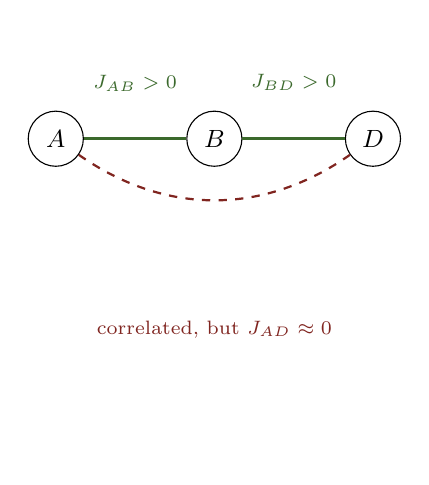
\begin{tikzpicture}[node distance=13mm, every node/.style={circle, draw, minimum size=7mm, font=\small}]
  \node (A) {$A$}; \node (B) [right=of A] {$B$}; \node (D) [right=of B] {$D$};
  \draw[maingreen!60!black, very thick] (A) -- (B) node[midway, above, draw=none, fill=none, font=\scriptsize]{$J_{AB}>0$};
  \draw[maingreen!60!black, very thick] (B) -- (D) node[midway, above, draw=none, fill=none, font=\scriptsize]{$J_{BD}>0$};
  \draw[mainred!70!black, dashed, thick] (A) to[bend right=35] node[midway, below, draw=none, fill=none, font=\scriptsize]{correlated, but $J_{AD}\approx 0$} (D);
\end{tikzpicture}
\end{center}
\vspace{-2pt}
The dashed link is the \emph{transitive trap}: $A$ and $D$ co-vary only because both couple to
$B$. Raw correlation reports it; DCA sets $J_{AD}\approx 0$.

\begin{warningbox}[Two confounders any generative model must respect]
\textbf{(1) Shared ancestry.} Species are not independent draws. In the toy data, if
$\{s_1..s_4\}$ form one clade, a \emph{single} loss of $A$ (and of $B$) in the ancestor of
$\{s_5,s_6\}$ explains their profiles --- the $A$--$B$ ``coupling'' could be two genes that
happen to be clade-restricted. Fixes: model gain/loss \emph{on branches} and/or weight
species by the tree. \textbf{(2) Transitivity} (the dashed edge above): pairwise statistics
conflate direct and indirect links; only a global (Potts) fit separates them.
\end{warningbox}

% ═══════════════════════════════════════════════════════════════════════════════
\section{Generating non-independence in ZOMBI2}
% ═══════════════════════════════════════════════════════════════════════════════

We want the forward gene-family process to \emph{produce} profiles whose fitted $J$ is the one
we chose. Three designs, increasing in fidelity to the Potts target.

\textbf{(a) Pathway membership + completeness-dependent rates (mechanistic).} Assign families
to pathways. Make a family's loss rate rise (and/or its gain rate fall) when its pathway is
incomplete, and vice-versa. Intuitive and biologically legible, and it naturally yields
``all-or-nothing'' pathways like $A,B$. Its coupling matrix $J$ is an \emph{emergent}
side-effect --- we would measure it, not set it.

\textbf{(b) Direct pairwise couplings via a coupled gain/loss process (Potts-faithful).} Here
we \emph{set} $h$ and $J$ and evolve the presence/absence vector $\sig$ along each branch as a
continuous-time Markov process whose \emph{stationary distribution is exactly the Boltzmann
$P(\sig)$ above}. This is Glauber/Gibbs dynamics. The clean recipe: define each family's
\emph{local field}
\[
f_i(\sig) \;=\; h_i + \sum_{j\neq i} J_{ij}\,\sigma_j ,
\qquad\text{and set}\qquad
\underbrace{\text{gain}_i = \rho\,e^{+f_i/2}}_{\text{if } \sigma_i=0},
\qquad
\underbrace{\text{loss}_i = \rho\,e^{-f_i/2}}_{\text{if } \sigma_i=1}.
\]
Then $\text{gain}_i/\text{loss}_i = e^{f_i}$, which is precisely the detailed-balance condition
for the Potts model, so the process relaxes to $P(\sig)$. Interpretation: when a partner $j$
(with $J_{ij}>0$) is present, family $i$ becomes easier to gain and harder to lose ---
mechanical co-occurrence. $\rho$ is an overall clock.

\textbf{(c) Hybrid (recommended starting point).} Let pathways define the \emph{block
structure} of $J$: strong positive $J$ within a pathway, zero across pathways, optional
negative $J$ between alternative pathways. This keeps (a)'s interpretability while giving
(b)'s controllable, recoverable target.

\begin{conceptbox}[Why this fits ZOMBI2 with almost no new machinery]
Our rate seam is already \texttt{RateModel.event\_weights(genome, branch, time)}. A new
\texttt{PottsRates(RateModel)} would (i) read the genome's presence vector
$\sig=\texttt{genome.presence\_vector(order)}$ (already implemented), (ii) compute $f_i(\sig)$
from stored $h,J$, and (iii) return gain/loss weights per family via the formula above. Because
the simulator recomputes \texttt{event\_weights} after \emph{every} event, the process is
automatically state-dependent --- i.e.\ Glauber dynamics along the tree --- \textbf{with no
change to the simulator, sampler, tree, or output code}. This is the exact seam we built the
architecture around.
\end{conceptbox}

\begin{intuitionbox}[The validation experiment (inject $\to$ recover)]
1. Choose a $J$ (e.g.\ a few coupled blocks). 2. Simulate with \texttt{PottsRates} on a species
tree; take the extant \texttt{Profiles.tsv}. 3. Run inverse-Potts/DCA on those profiles to get
$\hat J$. \textbf{Success} $=$ $\hat J \approx J$ (high rank correlation; injected pairs top the
list). 4. Crucially, repeat with $J=0$ (independent families) as a null and confirm the
recovered coupling is near-zero \emph{and} that the true-$J$ signal survives phylogenetic
correction --- i.e.\ it exceeds what shared ancestry alone produces. That last check is what
makes the result meaningful rather than a tree artifact.
\end{intuitionbox}

\begin{faqbox}[Design questions I would like your read on]
\textbf{Q: What is a ``gain'' of an \emph{existing} family?} In today's ZOMBI2, families are
born by \emph{origination} (brand new) and copies move by \emph{transfer}; re-acquiring a
\emph{lost} family is not a first-class event. Coupling (b) needs a ``regain'' channel. Options:
treat gain as transfer-from-a-donor-that-has-it (keeps HGT mechanistic, but then coupling is
limited by donor availability), or add an explicit regain rate. Which do you prefer?\\[2pt]
\textbf{Q: Presence/absence vs copy number.} The Potts $\sigma_i$ is binary presence. Do we
couple on presence only, or should copy number (our richer state) feed the field $f_i$?\\[2pt]
\textbf{Q: Static vs branch-varying $J$.} Should couplings be constant, or change across the
tree (e.g.\ regime shifts)? Constant is simplest and matches the inference assumptions.
\end{faqbox}

% ═══════════════════════════════════════════════════════════════════════════════
\section{Where this leaves us}
% ═══════════════════════════════════════════════════════════════════════════════

The empirical target (correlated profiles), the model (Potts / Ising energy over
presence/absence), and the generative dynamics (a coupled gain/loss CTMC with the
detailed-balance rates above) form a single coherent story. The recommended path is the
\emph{hybrid} (c): pathway-structured $J$, simulated by Glauber dynamics through a
\texttt{PottsRates} rate model, validated by inject-and-recover with a phylogeny-corrected null.
The open decisions are biological, not architectural --- chiefly how a lost family is regained,
and whether copy number should enter the field. Those are the choices I would like your feedback
on before we write \texttt{PottsRates}.

\vspace{2pt}
\footnotesize\textit{Sources: this note is written from the three cited papers and standard
Ising/Potts/DCA background; specific benchmark numbers were not re-verified against the PDFs. If
you want exact figures or quotations pinned down, send the PDFs and I will tighten them.}

\end{document}
